\documentclass[11pt,envcountsect,aspectratio=169]{beamer} %handout pour polycopier, draft pour le brouillon
% \usetheme[secheader]{Boadilla}
\usetheme{Nogent}
\usepackage[utf8]{inputenc}
\usepackage[french]{babel}
\usepackage[T1]{fontenc}
\usepackage{amsmath}
\usepackage{amsfonts}
\usepackage{amssymb}
\usepackage{pgf,tikz}

\DeclareFontShape{T1}{cmss}{m}{sc}{<->ssub*cmss/m/n}{}

\author[Thomas S. \& Romain V.]{Thomas Saigre \& Romain Vallet}

\hypersetup{%
	bookmarksopen=false,
	pdfsubject={Projet optimisation M1 CSMI},
}





\newcommand{\frametitre}{\begin{frame}
	\begin{center}
	{\Large\bf \secname}
	\end{center}
	\end{frame}
}


\title{Résolution du problème isopérimétrique}
\subtitle{Projet optimisation \\ M1 CSMI \\ Université de Strasbourg}
%\setbeamercovered{transparent} 
%\setbeamertemplate{navigation symbols}{} 
%\logo{} 
%\institute{} 
\date{5 septembre 2020}  %%%% Mettre la date de présentation <----------- !!!!!




% Macros
\newcommand{\R}{\mathbb{R}}
\newcommand{\Z}{\mathbb{Z}}
\newcommand{\C}{\mathcal{C}}
\renewcommand{\d}{\mathrm{d}}
\renewcommand{\P}{\mathcal{P}}
\renewcommand{\phi}{\varphi}
\newcommand{\A}{\mathrm{Aire}}
\newcommand{\p}{\mathrm{Per}}
\newcommand{\IA}{\textsf{IA}}
\newcommand{\IP}{\textsf{IP}}
\renewcommand{\Im}{\mathrm{Im}}
\renewcommand{\ss}{\vspace*{\baselineskip}}

\definecolor{ttttff}{rgb}{0.2,0.2,1}
\definecolor{xdxdff}{rgb}{0.49,0.49,1}


\newcommand\thm[2]{%
	\begin{beamerboxesrounded}[upper=titreB,lower=texteB,shadow=true]{Théorème : #1}
		\it #2
	\end{beamerboxesrounded}
	\normalfont
}


\begin{document}


\begin{frame}[plain]
\titlepage
\end{frame}


% Introduction
\section[Introduction]{Introduction}


% \frametitre



\begin{frame}{Problème isopérimétrique}

\end{frame}





% Table de matières
\begin{frame}{Table des matières}
\tableofcontents[hideallsubsections]
\end{frame}




\section{Définition du problème isopérimétrique}




\section{Maximisation d'un surface à périmètre constant}
% Ici je pense qu'il n'y a pas besoin de remettre tout les détails, peut être juste mettre le résultat final. Dans le template beamer, il y a une fonction qui permet de faire des blocs
% \thm{Titre}{énoncé}
% Tu peux aussi faire des blocs colorés en utilisant
%		\begin{beamerboxesrounded}[upper=titreB,lower=texteB,shadow=true]{Titre}
%			Texte
%		\end{beamerboxesrounded}
% et changer les couleurs (il y a déjà vert et rouge de définis, il y a juste à modifier le B dans titreB et texteB)
%


\begin{frame}{Maximisation d'un surface à périmètre constant}



\end{frame}








\section{Le problème de Didon}


\subsection{Le problème}


\begin{frame}{Problème de la reine Didon}

	\begin{itemize}
		\item Les terres où elle pourra s'établir seront \og autant qu'il pourrait en tenir dans la peau d'un b\oe{}uf\fg{}
		\item Exemple de la ville de Cologne, au Moyen-Âge :
	\end{itemize}
	
	\begin{figure}
		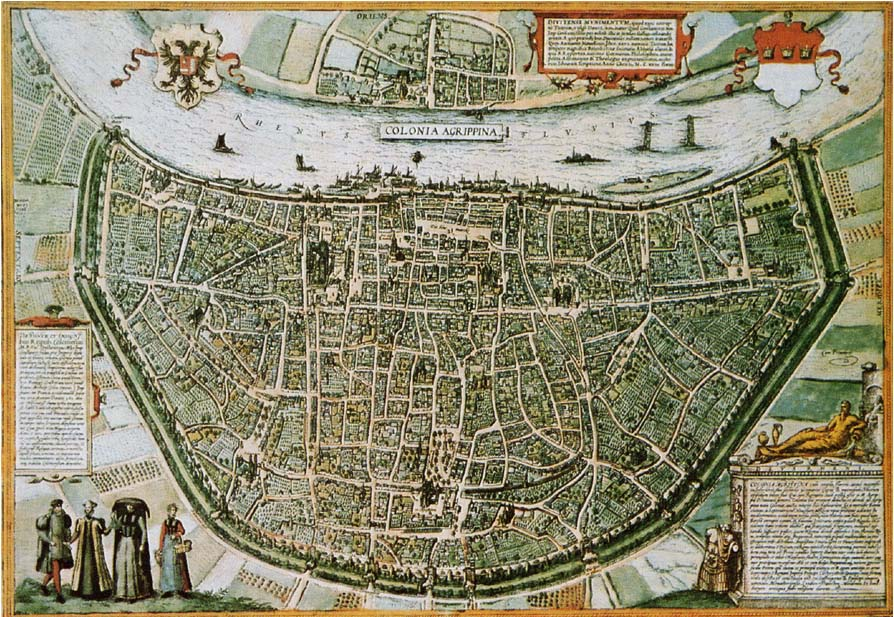
\includegraphics[scale=0.6]{img/cologne.jpg}
	\end{figure}

\end{frame}


\begin{frame}
	\frametitle{Position du problème}

	\begin{itemize}
		\item $\ell$ est fixé
		\item On cherche à maximiser du domaine pour un périmètre donné (ou de façon équivalente : minimiser le périmètre pour une aire donnée)
	\end{itemize}

	\begin{center}

		\begin{tikzpicture}
		\draw[->,color=black] (0,-0.5) -- (0,1);
		\fill[line width=0pt,color=ttttff,fill=ttttff,fill opacity=0.15] (-2,0) -- (2,0) -- (2,-0.5) -- (-2,-0.5) -- cycle;
		\begin{scriptsize}
		\fill [color=blue] (-2,0) circle (.5pt);
		\draw[color=blue] (-2,0) node[anchor=north] {$-\ell$};
		\fill [color=blue] (2,0) circle (.5pt);
		\draw[color=blue] (2.,0) node[anchor=north] {$+\ell$};
		\draw[color=black] (0,.8) node[anchor=south east] {$f$};
		\draw[color=ttttff] (0,-.5) node[anchor=south]{Mer};
		\end{scriptsize}
		\draw[smooth,samples=100,domain=-2.0:2.0] plot(\x,{0-((\x)-2)*((\x)+2)/5});
		\draw[->,color=black] (-2,0) -- (2,0);
		\end{tikzpicture}
		
		\end{center}

\end{frame}


\subsection{Résolution analytique}

\begin{frame}
	\frametitle{Résultat}

	\thm{}{%
		Le demi-cercle $y(x)=\sqrt{\ell^2-x^2}$ est solution du problème iso-aire en prenant $A_0=\frac{\pi}{2}\ell^2$. Il est donc solution du problème de Didon pour le choix de $p_0=\pi\ell$.
	}

\end{frame}





\subsection{Résolution numérique}

\begin{frame}
	\frametitle{titre}

	

\end{frame}




\subsection{Résultats}

\begin{frame}
	\frametitle{titre}

	

\end{frame}





\subsection{Autres méthodes de résolution}

\begin{frame}
	\frametitle{Autres méthodes de résolution}

	\begin{itemize}
		\item Lagrangien augmenté
		\item Pénalisation
		\item \dots
	\end{itemize}

\end{frame}





\end{document}